% Answers the question:
% What are methods to learn dynamic models and what are the limitations

% connecting to motion planning by adding dynamic constraints to a planner in configuration space. 
\section{Interaction Approaches and Model Identification Methods}
\label{section: interaction_approaches_and_model_iden_methods}
% introduce most prominent types of controllers
This section will describe the most prominent control methods which are applicable for controlling single- or multi-bodies. In general controllers have 3 abilities, which are tracking a reference signal, stabilising a system or rejecting disturbances, a controller can focus on one or a combination of these 3 abilities. The controllers' goal in this literature lies in tracking a reference signal to lower the output error. In \cref{section: system_model_representation} single-body models and multi-body models were introduced, now their control versions are introduced. \textbf{Single-body control} is an interaction approach which learns a single-body model and controls a single-body. As a reminder, a single-body is an object which is assumed to be connected for all times. \textbf{Multi-body control} controls two or more single- or multi- bodies. A multi-body controller uses a multi-body model. For example, a mobile robot pushing a ball. A controller actuates the robot directly and the object indirectly via the robot. Another example is a controller actuating a robot arm with a gripper holding a box. Single-body control involves driving for mobile robots and moving for a fixed robot. Multi-body control involves the robot pushing an object. The ability to push greatly broadens the robot's capabilities. Objects which are too heavy to lift could potentially still be pushed, objects out of reach to grasp could be in reach to push, and a gripper holding an object can additionally push another object but cannot grasp two objects at the same time.\\

Existing literature presents several methods for model-based robot control. The most prominent and established techniques can be categorised as predictive methods such as \ac{MPC} and reactive methods such as \ac{PID} control. Literature shows 2 types of model-free methods, completely model-free methods which act directly on \ac{IO} data, and model-free methods which are provided with data, but not explicitly given any model. Such   methods service by analysing \ac{IO} data and using system identification to update a model, whilst a controller uses such a model simultaneously.\\

Extensive research on robot controllers from last decades has been categorised in \cref{mindmap: classify_controllers}. \Cref{table: summary_controllers} provides a more detailed overview of some interaction approaches. 

\begin{figure}[ht]
\label{mindmap: classify_controllers}
\centering
\resizebox{!}{11cm}{%
\begin{tikzpicture}[
        mindmap,
    concept color = myDarkColor,
    every node/.style = {concept},
    grow cyclic,
    level 1/.append style = {
        concept color = myLightColor,
        level distance = 4.4cm,
        % sibling angle = 120
    },
    level 2/.append style =  {
        concept color = myEvenLighterColor,
        level distance = 2.8cm,
        % sibling angle = 100
    }
]
\node  {Controller Classes}
    child [grow = 310]{node {Predictive Methods}
        child[grow=300]{node {\ac{MPC}}}
        child[grow=240]{node {\acs{MPPI}}}
    }
    child [grow = 0]{node {Intelligent methods}
        child[grow=30]{node {\scriptsize \hspace{-0.2cm} \shortstack[]{ Reinforcement\\Learning}}}
        child[grow=330]{node {\acs{LSTM}}}
    }
    child [grow = 230]{node {Reactive methods}
        child[grow=300]{node {\ac{PID}}}
        child[grow=240]{node {Active Inference}}
    };
\end{tikzpicture}
}
\caption{A mind map showing the classification of control methods investigated in this literature. The first level of children displays the control classes, and the second level displays examples of the control classes \cite{mehra_map_2022}}
\end{figure}


% discuss all PID related papers
\subsection{Reactive Methods}
\label{subsection: reactive_methods}
Historically reactive methods were the first to arise. A widely used control method is the \ac{PID} controller. It's widely used due to its simplicity, clear functionality and ease of implementation. Tuning a \ac{PID} controller can be split up into 3 tuning approaches. Heuristic-tuning, rule-based tuning and model-based tuning \cite{tools_explore_2022}. A heuristic tuning method is one where general rules are followed to obtain approximate or qualitative results. The trial-and-error method is an example of heuristic tuning. Heuristic tuning is a quick and easy method to obtain a reasonable result, finding good performance can be very time-consuming. Rule-based \ac{PID} tuning methods assume a certain process response to obtain easy mathematical formulas that enable the tuning of a \ac{PID} controller. Commonly used rule-based tuning methods are the Ziegler-Nichols, Chien, Hrones and Reswick tuning methods. Performance improves and some stability guarantees arise, however for rule-based tuning some prior process knowledge is required. Model-based tuning or optimization-based \ac{PID} tuning allows you to obtain your P, I, and D parameters optimally. Control objectives such as disturbance rejection and reference tracking together with a model of your system and the engineering specifications of the closed-loop behaviour determine the final set of tuning parameters. Optimal performance comes at the cost of full prior system knowledge. For single-object control, the heuristic and rule-based tuning methods can apply because for these tuning methods full system knowledge is not required. For multi-body control, only the heuristic method could apply. In recent years automatically tuning \ac{PID} gains with more complex methods has risen. Such as \cite{ahn_online_2009} showed, who tuned a \ac{PID} controller using fuzzy logic this shows reactive control methods can be used without the need for extensive prior knowledge of the system. \\

\ac{PID} control has been around for many years. As opposed to this classical approach, the active Inference (AI) controller has been developed in the last decade and finds its origin in the field of neuroscience. Neuroscientist Karl Friston combined action selection with \ac{PEM}, which created the free-energy principle \cite{friston_free-energy_2009}, \cite{friston_action_2010}. In the field of robotics, \cite{pezzato_novel_2020} proposed an AI controller and implemented it on a real system for the first time. The AI controller is implemented on a real system. The control approach is a model-free online joint space controller, which was implemented on a 7-DOF Panda robot arm. The controller adapted rapidly to a changing environment and accounted for additional Gaussian noise for the joint measurements. If the free-energy depends explicitly on the control actions, then AI can provide a excellent fault metric as \cite{baioumy_fault-tolerant_2021} and \cite{pezzato_active_2021} have shown. One of the current drawbacks with an AI controller, there does not yet exist a stability proof and the solution to which the controller converges might be a local minimum. 
 
% discuss all MPC related papers
\subsection{Predictive Methods}
\label{subsection: predictive_methods}
In recent literature involving predictive methods \acf{MPC} methods are dominating, before moving on to \ac{MPC} and variations of \ac{MPC}, \ac{MPC} will briefly be explained.  The basic concept of \ac{MPC} is to use a dynamic model to forecast system behaviour and optimise the forecast to produce the best decision for the control move at the current time. Models are therefore central to every form of \ac{MPC}. Because the optimal control move depends on the initial state of the dynamic system\cite{rawlings_model_2020}. A dynamical model can be presented in various forms, let's consider a familiar differential equation. 
$$ \frac{dx}{dt} = f(x(t), u(t)) $$
$$ y = h(x(t), u(t)) $$ 
$$ x(t_0) = x_0 $$

In which $x \in \mathbb{R}^n $ is the state, $u \in \mathbb{R}^m$ is the input, $y \in \mathbb{R}^p$ is the output, and $t \in \mathbb{R}$ is time. The initial condition specifies the value of the state $x$ at $t = t_0$, and a solution to the differential equation for time greater than $t_0$, $t \in \mathbb{R}_{\geq 0}$ is sought. If little knowledge about the internal structure of a system is available, it may be convenient to take another approach where the state is suppressed, no internal structure about the system is known and the focus lies only on the manipulable inputs and measurable outputs. As shown in \cref{figure: mpc_block_diagam}, consider the system $G(t)$ to be
the connection between $u$ and $y$. In this viewpoint, various system identification techniques are used, in which $u$ is manipulated and $y$ is measured \cite{rawlings_model_2020}. From the input-output relation, a system model is estimated or improved. The system model can be seen inside the \ac{MPC} controller block in \cref{figure: mpc_block_diagam}.\\

\begin{figure}[h]
\centering
\begin{tikzpicture}
% blocks
\node[draw,
    minimum width=2cm,
    minimum height=1.2cm,
    fill=myLightColor,
] (system) at (0,0){$G(t)$};
\node[draw,
    minimum width=5.5cm,
    minimum height=2cm,
    fill=myEvenLighterColor,
    below = 1cm of system,
    label=above:MPC controller,
] (controller) {};
% the blocks and arrows inside MPC
\node[draw, minimum width=2cm, below=3mm of controller.north, anchor=north, fill=myDarkColor] (optimisation) {Optimisation};
\node[draw, below=8mm of optimisation.south, anchor=south, fill=myDarkColor] (model) {System Model};
\path[-stealth]
        (model.east) edge[bend right=70] node[pos=0.5, right] {Predict} (optimisation.east)
        (optimisation.west) edge[bend right=70] node[pos=0.5, left] {Action}  (model.west);
% Arrows
\draw[-stealth] (controller.west) |- ($(controller.west) - (1,0mm) $) |- (system.west) 
node[near end, above]{$u(t)$};
\draw[stealth-] ([yshift=-0.3cm]controller.east) -- ++(3,0) node[midway, above](input){$y_{ref}(t)$, $p$, $\mathbb{X}$, $\mathbb{U}$, $\mathbb{Y}$};
\draw[-stealth] (system.east) -- ++ (5, 0) 
    node[midway](output){}node[midway,above]{$y(t)$};
    \draw [-stealth] (output.center) |- ([yshift=0.5cm]controller.east); 
\end{tikzpicture}
\caption{System $G(t)$ with input ${u}(t)$, output $y(t)$ and \acs{MPC} controller with input $y(t)$, reference signal $y_{ref}(t)$, parameterisation $p$ and constraint sets $\mathbb{X}$, $\mathbb{U}$, $\mathbb{Y}$} \label{figure: mpc_block_diagam} \end{figure}  

As indicated in the problem description in \cref{section: problem_description}, prior knowledge about the structure of the robot itself is known. Such structure can be specified in a parameterisable system model, in which the influence of inputs and current states describes the behaviour of states and outputs. Uncertain parameters have to be sought, such as the center of mass, mass, and diameter of wheels. These parameters reside in the parameterisation $p$, see \cref{equation: parameterisable_model}. \Cref{figure: mpc_block_diagam} shows the parameterisation $p$, for purely analytical system models the parameterisation is left empty. The following explanation about \ac{MPC} is best understood with the differential drive robot in mind from \cref{fig: 2D_representation_robot}, with single-body model \cref{equation: differential_equation_differential_robot}. Some states of the system might be inside an obstacle region, such a region is undesirable for the robot to be in or go toward. The robot states are allowed in free space, which is all space minus the obstacle region. The free space is specified as a state constrained set $\mathbb{X}$. Allowable input can be restricted by the input constraint set $\mathbb{U}$, a scenario in which input constraints are required is for example the maximum torque an engine produces at full throttle. Lastly, the set of allowed outputs is specified in the output constraint set $\mathbb{Y}$. State, input and output constraints must be respected during optimisation, the optimiser takes the state-, input- and output constraint sets $\mathbb{X}$, $\mathbb{U}$, $\mathbb{Y}$ and if feasible, finds an action sequence driving the system toward the reference signal while constraints are respected. The \ac{MPC} system model predicts future states where the system is steered toward as a result of input actions.\\

The optimisation minimises an objective function $V_{N}(x_{0}, y_{ref}, \mathbf{u}_{N}(0))$, where\\ $ \mathbf{u}_{N}(k) = (u_k, u_{k+1}, \dots , u_{k+N})$. The objective function takes the reference signal as an argument together with the initial state and the control input for the control horizon. The objective function then creates a weighted sum of some heuristic function. States and inputs resulting in outputs far from the reference signal are penalised more by the heuristic function than outputs closer to the reference signal. Because the objective function is a Lyapunov function, it has the property that, it has a global minimum for the optimal input $\mathbf{u}_{N}^*$. If the system output reaches the reference signal $y_{ref}$, $x_{ref}$ then $u_{ref}$ will be mapped to the output reference signal as such $y_{ref} = h(x_{ref}, u_{ref})$. As a result solving the minimisation problem displayed in \cref{equation: mpc_problem} gives the optimal input which steers the system toward the output reference signal while at the same time respecting the constraints. 


\begin{mini}
{u_k, u_{k+1}, \dots , u_{k+N}} {
V_{N}(x_{0}, y_{ref}, u_k, u_{k+1}, \dots , u_{k+N})
}
{}{}
\addConstraint{x(k+1) = f(x(k), u(k))}
\addConstraint{x \in \mathbb{X}}
\addConstraint{u \in \mathbb{U}}
\addConstraint{y \in \mathbb{Y}}
\addConstraint{x(0) = x_0}
\label{equation: mpc_problem}
\end{mini}

\Cref{figure: mpc_scheme_basic} displays the predicted output converging toward the constant output reference. After solving the minimisation problem, \cref{equation: mpc_problem}, the optimal input sequence is obtained $\mathbf{u}^*_N$ (given that the constraints are respected for such input), from which only the first input is executed for time step $k$ to $k+1$. Then all indices are shifted such that the previous time step $k+1$ becomes $k$, the output is measured and the reference signal, parameterisation, and constraints sets are updated and a new minimisation problem is created, which completes the cycle. Note that \cref{figure: mpc_block_diagam,figure: mpc_scheme_basic} is an example \ac{MPC} controller, which hardly scratched the surface of \ac{MPC}, there are many variations and additions such as deterministic and stochastic \ac{MPC}, stage and terminal cost, distributed \ac{MPC}, etc. which \cite{rawlings_model_2020} visits extensively. 

\begin{figure}[h]
    \centering
    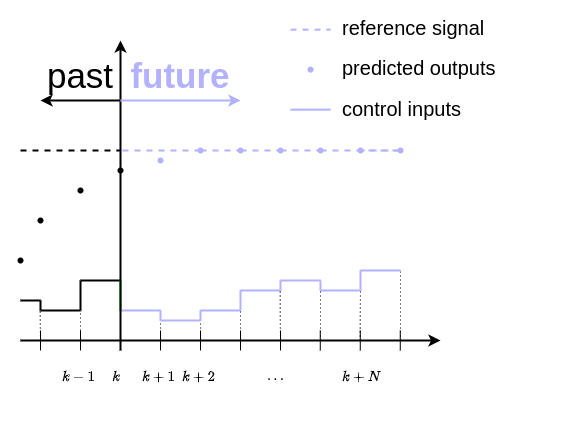
\includegraphics[width=0.8\textwidth]{figures/MPC_simple_diagram.png}
    \caption{A discrete \acs{MPC} scheme tracking a constant reference signal. $k$ indicates the discrete time step, $N$ the control horizon}
    \label{figure: mpc_scheme_basic}
\end{figure}

A major flaw for \ac{MPC} was the computation time required to solve a minimisation problem every time step. Because processors' power has increased, the \ac{MPC} framework can be applied in real time and is applicable for robotics. When applied to tracking a reference signal the \ac{MPC} framework outperforms classic control approaches such as \ac{PID} control \cite{nascimento_nonholonomic_2018}. Where \ac{MPC} excels at is tracking multiple objectives which can be weighted in the objective function. For example, \ac{MPC} can primarily track a robot path, while secondarily satisfying some additional dynamic specifications. This makes \ac{MPC} especially suitable in path tracking for nonholonomic robots. By restricting the state constraint set, obstacles can be avoided, such obstacles can even be avoided online  because the state constraint set may be changed during execution. It should however be feasible to find an input which satisfies all constraints. Because of its ease of tuning, handling multiple objectives, and flexibility in adding constraints, \ac{MPC} became the baseline standard to compare new control approaches with in control research. By now, linear \ac{MPC} theory is quite mature, and important issues
such as stability are well addressed in the last decade. Nevertheless, some systems are, in general,
inherently nonlinear. Therefore, especially in highly dynamic systems such as mobile robotics, linear
models are often inadequate to describe the process dynamics and nonlinear models have to be used. Thus nonlinear \ac{MPC} theory is required for which closed-loop stability proofs are lacking \cite{nascimento_nonholonomic_2018}. \\

Now the reader has gained a basic understanding of the workings of \ac{MPC} let's see relevant literature in the context of robot control in an environment with unknown objects. Starting with the literature accompanying single-body control.

\subsubsection*{(Integrated) Prediction Error Minimisation}
As mentioned models are central in every form om \ac{MPC}, so obtaining models is very important. \Cref{figure: mpc_block_diagam} displays a system model inside the block diagram used by the \ac{MPC} controller. The \ac{MPC} framework is flexible in handling different types of models, it accepts analytical, data-driven or hybrid forms. The \ac{MPC} controller's performance heavily relies on the accuracy of the system model. Having an accurate system model is thus crucial in the \ac{MPC} framework. One major system identification technique is the \ac{PEM} approach, it is the core of black-box identification methods \cite{farina_convergence_2008}. Generally in \ac{PEM} methods, the objective is to determine, from a finite number of measurements of the input and output sequences, a one-step-ahead predictor without prior system knowledge, or the system and covariance matrices of stochastic disturbances. The creation of an estimated model yields a state-space model or a transfer function model from which predictions can be made. \cite{verhaegen_filtering_2007}. An example is used to further clarify \ac{PEM} methods.

\subsection{Example Identification Method}
\begin{figure}[h]
\centering
\begin{tikzpicture}
% H, G and State-Space blocks
\node[draw,
    minimum width=2cm,
    minimum height=1.2cm,
    fill=myLightColor,
] (H) at (0,0){$H(q)$};
\node[draw,
    minimum width=2cm,
    minimum height=1.2cm,
    fill=myLightColor,
    below left =1cm of H,
] (G) {$G(q)$};
\node[draw,
    minimum width=3.5cm,
    minimum height=2cm,
    fill=myEvenLighterColor,
    below left= 1cm and -3.5cm of G,
] (SS) {\shortstack[l]{$A(p)$, $B(p)$, $K(p)$\\ $C(p)$, $D(p)$}};
%  two sum shapes
\node[draw, circle, minimum size=0.6cm, below= 1cm of H,] (sum) {};
\draw (sum.north east) -- (sum.south west)
    (sum.north west) -- (sum.south east);
\draw (sum.north east) -- (sum.south west)
(sum.north west) -- (sum.south east);
\node[left=-1pt] at (sum.center){\tiny $+$};
\node[above] at (sum.center){\tiny $+$};
\node[draw, circle, minimum size=0.6cm,below right= 0.4cm and 4cm of G] (pm) {};
\draw (pm.north west) -- (pm.south east);
\draw (pm.north east) -- (pm.south west)
(pm.north west) -- (pm.south east);
\node[above] at (pm.center){\tiny $-$};
\node[below] at (pm.center){\tiny $+$};
\draw[-stealth] (H.south) -| (sum.north);
\draw[-stealth] (G.east) -- (sum.west);
% every arrow 
\draw[-stealth] (sum.east) -| (pm.north)
node[midway](output){}node[midway,above]{$y(k)$};
\draw[-stealth] ($(output.center) - (1,0mm)$) |- ++(0,-1) -| ($([yshift=0.5cm]SS.west) - (1,0mm) $) -- ([yshift=0.5cm]SS.west);
\draw[stealth-] (G.west) -- ++(-3, 0)
node[](input){}node[midway, above]{$u(k)$};
\draw[-stealth] ($(input.center) + (1,0mm)$) |- ([yshift=-0.5cm]SS.west);
\draw[-stealth] (SS.east) -| (pm.south)
node[midway, below] {$\hat{y}(k, p)$};
\draw[-stealth] (pm.east) -- ++ (1,0)
node[near end, above] {$\epsilon(k,p)$};
\draw[stealth-] (H.west) -- ++ (-1,0) node[midway, above] {$e(k)$};
\end{tikzpicture}
\caption{A block diagram displaying the structure of the prediction-error model-estimation method \cite{verhaegen_filtering_2007}}
\label{figure: pem_block_diagram} \end{figure}  

\Cref{figure: pem_block_diagram} displays a block diagram of the prediction-error model-estimation method. Here output $y(k)$ is created by summing system $G(q)u(k)$ with additional noise $H(q)e(k)$, the input $u(t)$ is stochastically independent of $e(k)$ a zero-mean white-noise sequence. The one-step-ahead predictor tunes the state matrices $A(p)$, $B(p)$, $K(p)$, $C(p)$, $D(p)$ such that the output error $\epsilon(k,p)$ is minimised.

Two important assumptions are: $G(q)$ is an \ac{LTI} system, and the stationary one-step-ahead predictor displayed in \cref{equation: verhaegen_one_step_ahead} is of known order.
In this example the goal is to obtain the state-space matrices from input-output data. \Cref{figure: pem_block_diagram} displays a block diagram of the \ac{PEM} methods. With input-output data generated as:

\begin{equ}[!ht]
\begin{equation}
y(k) = G(q)u(k) + H(q)e(k)
\label{equation: verhaegen_signal_generating}
\end{equation}
\caption*{A signal-generating system, it's input-output data is to be used for identification. $G(q)$ represents the deterministic part and $H(q)$ the stochastic part of the system, both $G(q)$ and $H(q)$ are discrete transfer function models, from \cite{verhaegen_filtering_2007}}
\end{equ}

The one-step-ahead predictor of known order takes, for a state-space model the following form:
\begin{equ}[!ht]
\begin{equation}
\begin{aligned}
\hat{x}(k+1) &=A \hat{x}(k)+B u(k)+K(y(k)-C \hat{x}(k)-D u(k)), \\
\hat{y}(k) &=C \hat{x}(k)+D u(k)
\end{aligned}
\label{equation: verhaegen_one_step_ahead}
\end{equation}
\caption*{Given a finite number of samples of the input signal $u(k)$ and the output signal $y(k)$, and the order of the predictor. The goal is to estimate the system matrices $A$, $B$, $C$, $D$ and $K$ in this predictor such that the output $\hat{y}(k)$ approximates the output of \cref{equation: verhaegen_signal_generating}}
\end{equ}

A parameterisation of the one-step-ahead predictor as a stationary Kalman filter, \cref{equation: verhaegen_one_step_ahead} with parameterisation $p$ and the one-step-ahead predictor of the previous time step gives the parameterised one-step-ahead predictor:

\begin{align*}
\hat{x}(k+1|k, p) &= (A(p)-K(p)C(p))\hat{x}(k|k-1,p) + (B(p)-K(p)D(p))u(k) + K(p)y(k)\\ \hat{y}(k|k-1, p) &= C(p)\hat{x}(k|k-1, p)  + D(p)u(k)
\end{align*}

By minimising the output error $y(k) - \hat{y}(k|k-1,p)$ an optimal parameterisation is be found, such a parameterisation together with its parameterisable one-step-ahead predictor can be used by the \ac{MPC} framework. Chapter 8, \cite{verhaegen_filtering_2007} can elaborate further on \ac{PEM} methods with subjects such as the ARMAX, ARX and Box-Jenkins parameterisation, the innovation model or closed-loop system behaviour. \ac{PEM} system identification techniques rely on \ac{IO} data, which must contain enough information, which in robotics can be an issue, since there is not always time to collect a rich enough \ac{IO} data set. Though, \ac{PEM} methods can with little prior knowledge formulate an accurate system model, if provided with enough \ac{IO} data. \cite{farina_convergence_2008} has compared single- and multistep \ac{PEM} methods and convergence properties in a predictive control context, and provided proof that showing that single step and multistep \ac{PEM} methods yield unbiased models. This allows the conclusion that \ac{PEM} methods are proper methods to estimate a linear system model, provided that there is access to enough information-rich \ac{IO} data of such a system. \ac{PEM} assumes the true dynamics can be estimated accurately with an \ac{LTI} system, \ac{PEM} methods are ideal for single-body control. \ac{PEM} for multi-body control is feasible, but not ideal since multi-body control is too nonlinear to be properly captured using an \ac{LTI}-based system identification method.\\

An improvement on \ac{PEM} which lacks capturing changing dynamics, was made by \cite{seegmiller_vehicle_2013} where a system model is parameterised using \ac{IPEM}. The idea is to integrate the left-hand side $\frac{dx}{dy}$ of the system dynamics, resulting in some favourable effects. \ac{IPEM} can calibrate offline (slip) and online (odometry), \ac{IPEM} improves upon \ac{PEM} by using only low-frequency measurements, and fewer ground truth measurements and slip can be accounted for. These plus points come at the cost of additional complexity.
Because fewer measurements are required, \ac{IPEM} detects and adjusts faster to changing system dynamics, which makes \ac{IPEM} more suitable for robotic applications compared to \ac{PEM}. Additionally \ac{PEM} assumes an \ac{LTI} system, where \ac{IPEM} claims to converge for a linear time-variant system, broadening the set of systems \ac{IPEM} can model. Especially for the following situation which is described in \cite{seegmiller_vehicle_2013}. A robot plans to make an aggressive turn into a narrow corridor, however, due to unmodeled understeering, the
robot actually makes a wider than expected turn driving into the wall of the corridor. The robot has deviated from the planned path. Based on position feedback, the robot
compensates by planning a sharper turn. Once again, the robot fails to execute the planned path as its curvature exceeds the limits
of the steering mechanism. The robot must now abandon the attempt and drive in reverse to avoid a collision. If the planner had an
accurate model, it would have simply turned harder at the beginning of the turn when the turn was still feasible.\\

\ac{IPEM} methods are ideal for estimating rapid-changing true dynamics with a stochastic nature, arising during tracking of a reference for a mobile robot with additional measurement noise. The mobile driving robot can be modelled as a linear time-variant model which accounts for slip and odometry changes.\\

\ac{PEM} and \ac{IPEM} are suitable for single-body models because single-body systems can be simplified to an \ac{LTI} system. Multi-body systems cannot since they are dominated by nonlinear dynamics. Multi-body system thus require a different system identification method, recent literature reveals that a set of test pushes is the dominant data collection method for gathering a set of \ac{IO} data. As the name "test pushes" suggests, data collection focuses on push manipulations and is collected by the robot performing several test pushes against the object from different angles. The push is taken as input, and the location of velocity of the object is taken as output to form a train set. From this train set, there exist multiple methods to create a system model. Let's review recent literature,  for every new object, \cite{mericli_push-manipulation_2015} creates, a sequence of random push actions and the effect of the push. A 3-dimensional Gaussian distribution (for 2D pose variables $x$, $y$ and $\theta$) is fitted on the sample pushes. The Gaussian distribution can be used as a one-step-ahead predictor used for control. A disadvantage of \cite{mericli_push-manipulation_2015} is, after every push the object comes to a complete stop. A sequence of pushes is generated and executed in a push-stop-push-stop fashion, which could be one continuous push. \cite{bauza_data-efficient_2018} overcomes this problem by converting the Gaussian process to linearized motion equations which can be directly fed into the \ac{MPC}. Both \cite{mericli_push-manipulation_2015} and \cite{bauza_data-efficient_2018} use data-driven approaches, \cite{bauza_data-efficient_2018} additionally has an analytical approach. Initially, an analytical approach has the lowest tracking error, after $\sim 100$ number of tests pushes the data-driven approaches outperform analytical approaches because the push analytical models does model the more nonlinear parts of the true dynamics. Such as small variations in the sliding friction or the mass distribution. \cite{bauza_data-efficient_2018} did show a data-driven stable controller can be created after only $\sim 10$ test pushes. \\  

In the \ac{MPC} frameworks, several single- and multi-body methods are discussed, transitioning from single-body control to multi-body control can causes problems. Single-body control requires the constraints which belong to a single-body model, when single-body control switches to multi-body control the dynamical and kinematic constraints should update such that the multi-body constraints are respected. This discontinuity of model dynamics introduces control and planning problems. Control issues arisen during discrete dynamic models are now discussed, the arisen problems affecting planning will be discussed in the next chapter.\\

\subsubsection*{Reactive \ac{MPC}}
As \cite{toussaint_sequence--constraints_2022} describes in their problem description: \ac{TAMP} plans include switches in kinematic and dynamic constraints, and the original plan might provide temporal scheduling of such switches. However, for reactive execution the exact timing of constraint switches needs to be reactive, which either requires employing optimization methods invariant to such switches \cite{toussaint_differentiable_2019}, \cite{posa_direct_2014} or include explicit timing-estimation and -optimization as part of the \ac{MPC} problem.\\

The solution proposed by \cite{toussaint_sequence--constraints_2022} is to take the timing of switching constraints as a decision variable yielding a timing-optimal sequence-of-constraints \ac{MPC}. Because the reactive \ac{MPC} can work with somewhat accurate system models, the reactive  \ac{MPC} controller is ideal for objects for which a not very accurate model of the true dynamics is only available. The reactive behaviour makes the control algorithm well suited for pushing and avoiding collision of incoming objects. A disadvantage in reactive \ac{MPC} is the CPU power it requires to run, another drawback is that a reactive \ac{MPC} is unable to learn any system model, the reactive controller cannot give any guarantees when operating on unknown objects. However, if a (potentially inaccurate) single-and multi-body model for is provided the reactive \ac{MPC} can successfully perform push manipulations. Single- and multi-body models obtained by different system identification methods can be combined with a reactive \ac{MPC} controller. 

% find MPPI interesting
\subsubsection*{Model Predictive Path Integral Control}
Introduced by \cite{williams_model_2015} \ac{MPPI} control arose. Which was followed by \ac{MPPI} control combined with various system models, identification methods \cite{abraham_model-based_2020}, \cite{cong_self-adapting_2020}, \cite{arruda_uncertainty_2017}. The core idea is from the current state of the system with the use of a system model and randomly sampled inputs to simulate in the future a number of "rollouts" for a specific time horizon, \cite{neuromorphic_tutorial_ltc21_2021}. These rollouts indicate the future states of the system if the randomly sampled inputs would be applied to the system, the future states can be evaluated by a cost function which penalised undesired states and rewards desired future states. A weighted sum over all rollouts determines the input which will be applied to the system. If a goal state is not reached, the control loop starts with the next iteration. An example is provided, see  \cref{figure: mppi_car_with_rollouts}. 

\begin{figure}[h]
    \centering
    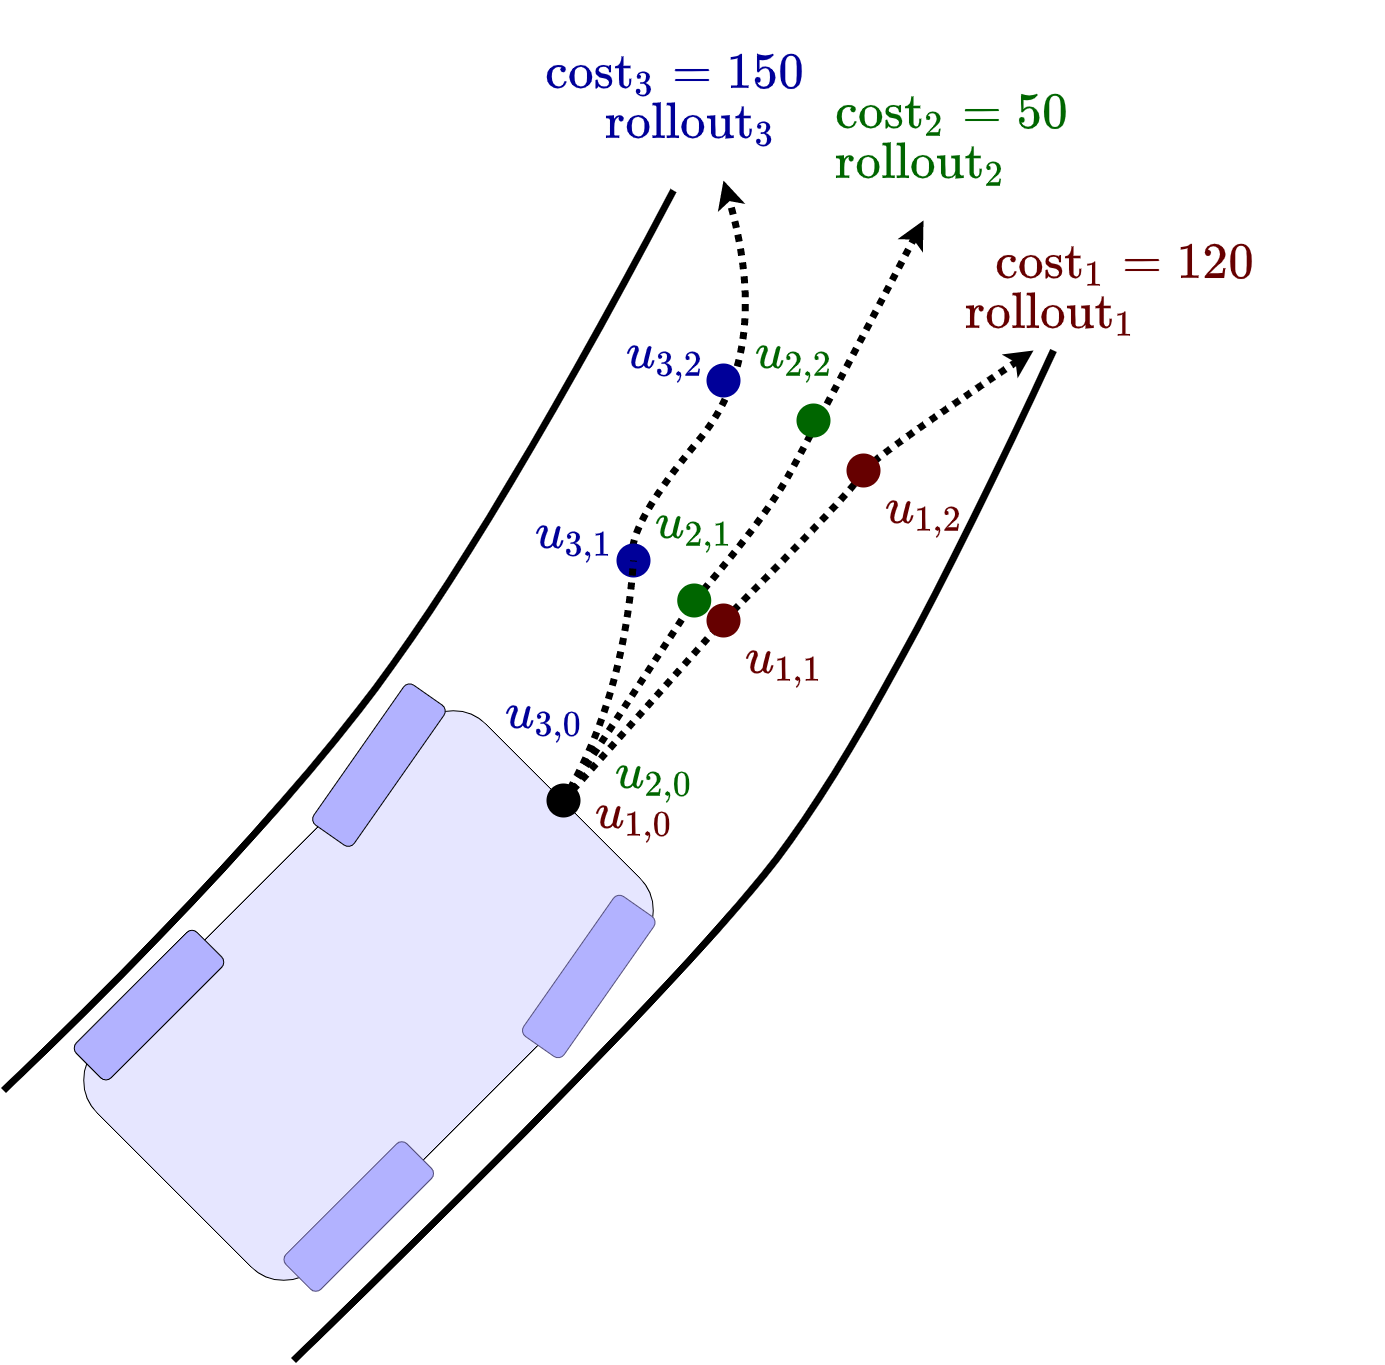
\includegraphics[width=0.5\textwidth]{figures/MPPI_car_with_rollouts.png}
    \caption{\acs{MPPI} controlled race car using a control horizon of 3 time steps, with 3 rollouts all having their respected inputs as $u_{i,j}$ where $i$ is the rollout index and $j$ indicates the time step \cite{neuromorphic_tutorial_ltc21_2021}.}
    \label{figure: mppi_car_with_rollouts}
\end{figure}

Here 3 rollouts are displayed, The objective function is designed to keep the car driving on the center of the road by penalising rollouts which are further away from the center of the road relatively more. resulting in a high cost for $\text{rollout}_1$ and $\text{rollout}_3$ compared to $\text{rollout}_2$. As a result, the input send to the system as a weighted sum of the rollouts is mostly determined by $\text{rollout}_2$. The weighted sum determining the input is displayed in \cref{equation: mppi_weighted_sum}, from \cite{neuromorphic_tutorial_ltc21_2021}.

\begin{equation}
u(k+1)=u(k)+\frac{\sum_{i} w_{i} \delta u_{i}}{\sum_{i} w_{i}}
\label{equation: mppi_weighted_sum}
\end{equation}

Where $\delta u_i$ is the difference between $u(k)$ and the input for rollout $i$, the weight of $\text{rollout}_i$ is detemined as: $w_{i}=e^{-\frac{1}{\lambda} \text{cost}_{i}}$, $\lambda$ is a constant parameter. The reader is now somewhat familiar with the \ac{MPPI} concept, Now some applications with \ac{MPPI} and multi-object control are discussed.\\

From a test pushes train set, \cite{arruda_uncertainty_2017} creates a forward model. The forward model is based on a Gaussian process and can sample multiple trajectories or rollouts in the future, these rollouts are then sent to the \ac{MPPI} controller. While \cite{arruda_uncertainty_2017} was able to create a forward model from scratch, it was unable to improve the forward model after the training phase. This strategy is ideal when the true push dynamics are fully unknown, but makes it less ideal when dynamics change over time.\\

\cite{abraham_model-based_2020} proposed an \ac{EMPPI} controller which requires a partially unknown parameterisable system model of the robot and objects in the environment. Thus this method is as opposed to \cite{arruda_uncertainty_2017} not data-driven. If such a model is provided, \ac{EMPPI} constantly improves the parameterisation found during execution. Which is accomplished by recursively searching for a parameterisation for the partly known dynamics. It is however assumed that the true dynamics reside in the local minima of the parameterisation.\\

Both model identifying methods used in combination with a \ac{MPPI} controller mentioned above need a training set obtained by test pushes. The training phase can only be over when the model results in a stable closed-loop controller. The capability to yield a stable controller is crucial in robotics where time and resources are limited. Currently the fastest stable controller for push manipulation was proposed by \cite{bauza_data-efficient_2018} where the train set required a minimum of only $\sim 10$ train pushes. Then \cite{cong_self-adapting_2020} even claims to require less than 5 train pushes. With the use of a recurrent \ac{LSTM} based model to predict the motion of objects with unknown parameters. The \ac{LSTM}  model provides the \ac{RMPPI} controller with motion predictions. By updating the \ac{LSTM} model and executing \ac{RMPPI} control at the same time the algorithm is self-adapting.\\

\ac{MPPI} has some advantages in comparison to \ac{MPC}. \ac{MPPI} can be optimised by running multiple simulations in parallel. Parallel optimisation improves converging to a control policy \cite{williams_model_2017}. \ac{MPPI} is based on stochastic sampling, this makes the \ac{MPPI} controller naturally take into account nonlinear dynamics, and incorporate nonsmooth/non- differentiable cost functions without approximations \cite{williams_model_2015}, which makes \ac{MPPI} very applicable for multi-body control where the true dynamics mainly are nonlinear. \\ 

\subsection{Intelligent Methods}
\label{subsection: intelligent_methods}
Already seen in previous subsection paper \cite{cong_self-adapting_2020} used a predictive method for control. To identify the system, an intelligent \ac{LSTM} method was used. Intelligent system identification method are seen more often in recent literature, so has \cite{scholz_learning_2015} shown multi-body control using a physics-based reinforcement learning approach. A key advantage intelligent methods provide is the learning speed intelligent methods offer, online adaption is for both \cite{cong_self-adapting_2020} and \cite{scholz_learning_2015} a major advantage over other methods, which makes them very suitable for learning dynamic properties of objects with unknown dynamics. However intelligent methods are out of the scope of this literature because they have trouble generalising. To elaborate, intelligent methods perform very well on the train set, but on unseen data intelligent methods lack performance. The entire point of learning is to be able to generalise to the unseen, even out-of-distribution, and it is currently very difficult to assess learning performance on novel tasks \cite{roy_machine_2021}.\\

Control and identification methods investigated in this literature are conveniently summarised in the following table:

%% TABLE %%%
\begin{table}[H]
\centering
\ra{1.3}
\begin{tabular}{@{}lllllcl@{}}
\rotatebox{30}{\parbox{1.3cm}{System Iden. Type}} & \rotatebox{30}{\parbox{1cm}{Controller Type}} & \rotatebox{30}{\parbox{1.2cm}{Sources}} & \rotatebox{30}{\parbox{1.2cm}{\parbox{1.3cm}{Single-/Multi-body model}}} &  \rotatebox{30}{Requires} &   \rotatebox{30}{ \parbox{1.5cm}{Online Adaptation Model}} &  \rotatebox{30}{\parbox{1.3cm}{Type of model Stored}} \\
\midrule
\multicolumn{4}{l}{\textit{Single-Body Control}} &&&\\
\rowcolor{myEvenLighterColor}  &&&&&&\\[-11pt]
\rowcolor{myEvenLighterColor} &  \shortstack[l]{Fuzzy\\Control\\ \& \ac{PID}}& \cite{ahn_online_2009} & Single  & \shortstack[l]{initial PID\\gains} 
& \cmark & \ac{PID} gains \\
&&&&&&\\[-11pt]
\shortstack[l]{\ac{PEM},\\\ac{IPEM}} & \ac{MPC} & \cite{seegmiller_vehicle_2013}, \cite{farina_convergence_2008} & Single & \shortstack[l]{Nonlinear \\ differential \\ equation}  & \cmark & \shortstack[l]{Calibrated \\nonlinear \\ differential \\ equation} \\
\rowcolor{myEvenLighterColor}  &&&&&&\\[-11pt]
\rowcolor{myEvenLighterColor} - & \shortstack[]{Active\\Inference} & \cite{pezzato_novel_2020}  & Single &   \shortstack[l]{initial\\AI controller\\parameters} & \cmark  & 
\shortstack[l]{belief\\dynamics}\\
\midrule
\multicolumn{2}{l}{\textit{Multi-Body Control}} & & & & &\\
\rowcolor{myEvenLighterColor}  &&&&&&\\[-11pt]
\rowcolor{myEvenLighterColor} - & \shortstack[l]{Reactive\\\ac{MPC}} &\cite{toussaint_sequence--constraints_2022} & \shortstack[l]{Single,\\ Multi} & \shortstack[l]{Dynamical\\model} & \xmark & - \\
 &&&&&&\\[-11pt]
\shortstack[]{Model\\Fitting} & \ac{MPC} &\cite{mericli_push-manipulation_2015}, \cite{bauza_data-efficient_2018} & Multi & \shortstack[l]{sample \\ pushes} & \xmark & \shortstack[]{3D Gaussian\\distribution} \\
\rowcolor{myEvenLighterColor} &&&&&&\\[-11pt]
\rowcolor{myEvenLighterColor}- & unknown &\cite{stuber_feature-based_2018} & Multi & \shortstack[l]{3D object \\point cloud,\\ test pushes}  & \xmark & \shortstack[]{Contact\\model} \\
&&&&&&\\[-11pt]
- & \ac{EMPPI} &\cite{abraham_model-based_2020} & Multi & \shortstack[l]{Partially\\ Unknown\\Dynamics}& \cmark & \shortstack[l]{tuning\\parameters\\Stochastic\\Dynamics}\\
\rowcolor{myEvenLighterColor}  &&&&&&\\[-11pt]
\rowcolor{myEvenLighterColor} \ac{LSTM} & \ac{RMPPI} &\cite{cong_self-adapting_2020} & Multi &   \shortstack[l]{warm up stage,\\contact point} & \cmark & \ac{LSTM}\\
&&&&&&\\[-11pt]
\shortstack[]{Physic-\\based\\Regrssion} & - &\cite{scholz_learning_2015} & Multi & \shortstack[l]{Gripper\\Torques\\for all $t$}& \cmark & \shortstack[l]{Policy}\\
\bottomrule
\end{tabular}
\caption{Summary of interaction approaches and identification methods. The first column displays the model used by the controller, if no model identification method is used this is indicated with a "-". Prior knowledge is indicated in the "Requires" column, poses for single- and multi-bodies are assumed to be known for all time steps. The parameters used to fully store the model are indicated in the last column. }
\label{table: summary_controllers}
\end{table}

\section{Discussion}
\label{section: controllers_discussion}
In \cref{section: system_model_representation} a categorisation of system models is made which are the analytical, data-driven models and hybrid models. Analytical models could be used in situations where a system is fully analysed. Even the robot itself cannot be fully analysed because of slowly changing true dynamics let alone any of the unknown objects. Analytic approaches are for this reason excluded from further investigation. Better suited is the data-driven approach where, with enough data nonlinear parts of the true dynamics are captured, given that enough data is collected and the nonlinear behaviour resides in the data collected. Whilst hybrid models quickly offer a stable model, data-driven models eventually outperform hybrid models. Assuming some structure of the true dynamics allows for obtaining a model fast, while losing from data-driven methods in accuracy during convergence. The hybrid approach is best suited for single-body models, while data-driven methods are best suited for multi-body models. \\

Multiple interaction approaches have been categorised, where predictive methods are the dominant methods. The predictive methods are able to incorporate constraints en uncertainty comparably well. Predictive methods performance heavily depends on the models they use, the system identification method is thus an important factor for stability and overall performance. \\

Many approaches have been discussed to learn dynamical models and their limitations have been emphasised, Because limitations are method-specific the challenge lies in when to choose which interaction approach and which system identification approach. For example, in push manipulation without any prior knowledge the only methods applicable are ones which start with data-driven system identification. Some objects might jump discontinuously between single- and multi-body dynamics (e.g. a ball) such a situation ask for a timing-optimal \ac{MPC}. Objects could be in a corner surrounded by walls, limiting the training phase to only perform test pushes from one side, the best candidate for such a situation would be \ac{LSTM} based controller which requires a minimum amount of training pushes. \\

There is no best interaction approach, different task required different approaches. Mainly the identification approach should be chosen specialised for the task at hand. For robot driving the \ac{MPC} control methods is best suited, using \ac{PEM} for mostly constant system dynamics and \ac{IPEM} for changing system dynamics. Multi-body systems are best controller using \ac{MPPI} control because they naturally incorporate the nonlinear mechanics, the modelling method should take nonlinearities into account, which are data-driven methods such as contact models, or a more complex methods such as \ac{LSTM}. 
